\documentclass[12pt]{article}

\usepackage{amsfonts}
\usepackage{amsmath}
\usepackage{graphicx}
\usepackage{lmodern}
\usepackage{hyperref}

\title{Ardana Rollups System Architecture}
\author{Ardana Labs}


\begin{document}


\maketitle


Ardana Rollups are a general purpose ZK rollup layer 2 scalability solution for Cardano. ZK rollups are a mechanism by which transactions are processed off-chain and the results of those transactions are published onto the blockchain using zero knowledge proofs. More precisely, ZK rollups use zkSNARKS, which are in other words zero knowledge succinct non-interactive arguments of knowledge. By moving data and processing off-chain, ZK rollups allow for higher throughput. By using a secure, decentralized layer 1 blockchain and zkSNARKS, ZK rollups inherit certain security properties of the layer 1 solution, namely that we need not assume that any party is trustworthy, and nobody is able to cause unlawful (protocol-violating) results to be produced on-chain. Additionally, Ardana Rollups are designed to have the security property that there is no single point of failure, meaning that there is no individual or organization whose ongoing participation is required for the proper, intended functioning of the solution.

ZK rollups are an increasingly popular choice of layer 2 solution on Ethereum, with multiple choices of ZK rollup solution available for use, including zkSync, StarkEx, and Loopring. \cite{ethworks-20} In contrast, Ardana knows of no prior art for a ZK rollup based layer 2 solution on Cardano. However, we believe that ZK rollups will be an important part of the Cardano ecosystem moving forward, just as they are in Ethereum today.

This is the system architecture document for Ardana Rollups. This defines the key components of Ardana Rollups and their interactions with each other and the outside world, as well as the rationale for those design decisions. This is different from a whitepaper or a technical spec in that it does not attempt to provide enough information to implement Ardana Rollups. Instead, you can think of it as a sketch. Technical specs will fill in the picture in much greater detail, sufficient to guide implementation, and a technical whitepaper will describe Ardana Rollups in a form more suitable for general consumption as compared to the specs.

\section{Background}

This section covers background information necessary to understand the design of Ardana Rollups and ZK rollup solutions more generally.

A blockchain uses a consensus algorithm executed by a decentralized network of nodes in order to process financial transactions and other information. Thanks to the consensus algorithm, parties can be assured that their money and other information assets stored on the blockchain will not be used in a manner they did not authorize, without a need to trust that any particular participant in the protocol is behaving honestly.

Blockchains are an important innovation in financial technology which have the potential to liberate humanity from centralized systems of finance. However, this will only be possible to the extent that blockchain developers can obtain massive scalability, such that these systems could actually replace the centralized financial technology which most people use most of the time to settle financial transactions electronically today. For example, Visa reportedly processes over 150 million transactions per day on average, and is capable of processing more than 24,000 transactions per second. \cite{visa}

Scalability of blockchain solutions is a widely recognized problem. There are a few angles of attack on this problem. One angle is to increase the transaction throughput of the blockchain itself. This is an important task but also a difficult one. Another angle is to multiply the number of blockchains in use, such as in the case of Kadena's Chainweb. \cite{chainweb} A third angle is to use so-called layer 2 solutions, whereby transactions are processed off-chain and then the results are later synced onto the chain. With layer 2 solutions, the blockchain can be used simply as a settlement layer, while application domain business logic lives off-chain and the amount of state and state changes stored on the chain can be greatly reduced.

ZK rollups are an example of a layer 2 solution strategy. ZK rollups make use of zkSNARKs. zkSNARKs are a type of proof. A proof, for our purposes, is a piece of information which evidences the truth of some statement. In the context of formal logic, a proof is in other words a sound argument, which is a valid argument where the premises are true. A valid argument, speaking informally, is an argument which in virtue of its logical structure guarantees that the conclusion is true provided that the premises are true. This is \emph{not}\/ what we mean by a proof here. A proof in this context is a piece of information whose existence demonstrates that there is only a negligible probability that the statement to be proven is not true. In this sense of the word proof, for example, an ED25519 signature is a proof that a person who has the private signing key ran the signing algorithm on the piece of information that was signed.

By definition, a zkSNARK is a zero knowledge succinct non-interactive argument of knowledge. In this definition, ``argument of knowledge'' means ``proof'' (in the sense of ``proof'' just stated). A zkSNARK has the characteristics of being zero knowledge (meaning it does not prove anything more than the statement to be proven), succinct (meaning the proof can be represented as a small number of bytes), and non-interactive (meaning the proof can be represented as a single message, as opposed to a multi-step interaction between the proving entity and proof-checking entity).

For our purposes, the most relevant characteristics of zkSNARKs are the succinctness and non-interactivity properties. It may be the case that we could get by with just SNARKs, i.e., succinct non-interactive proofs which are not necessarily zero-knowledge. However, we are using zkSNARKs for the reason that the bulk of the research on SNARKs is on zkSNARKs, and we believe that the most mature and relevant SNARK solutions available are zkSNARK solutions.

The reason that succinctness and non-interactivity are key properties here is that we need to store the proofs in transactions on the blockchain. Thus due to the nature of blockchain transactions, which are short single messages, the proofs must be succinct and non-interactive.

ZK rollups are in essence a simple concept. In a pure blockchain protocol (without a layer 2 solution), all transactions, all smart contract code, and all smart contract state data are normally stored on the blockchain. In a ZK rollup solution, some of this code and data gets stored off-chain, and instead the chain stores proofs that this information exists. The zkSNARKs stored on chain prove that for some set of inputs and some set of outputs, there exists a set of transactions which were signed by the relevant parties and which followed the rules of the relevant smart contracts. Those transactions never need to be recorded on the chain; we need only record the inputs, the outputs, and the proof that those outputs lawfully (according to the laws of the blockchain protocol) resulted from the inputs.

Due to the nature of zkSNARKs, this strategy allows for a potentially unlimited number of transactions to be performed with a constant $O(1)$ amount of on-chain information. Therefore this ZK rollup strategy allows for potentially very efficient usage of the limited information storage capacity of the blockchain. 

Similarly, the computational complexity of verifying a zkSNARK proof is $O(1)$, and therefore, the ZK rollup strategy allows for a potentially unlimited amount of computation to be done off-chain to validate transactions which are all verified by a single proof, and the on-chain computation required to validate those transactions is limited to the relatively small and $O(1)$ amount of computation required to check the proof. This makes for a potentially very efficient usage of the limited computational capacity of the blockchain.

Blockchains are one type of decentralized data store, but there are also other types of decentralized data stores which are not blockchains. A blockchain is a distributed ledger with a consensus algorithm. The two main ingredients in that concept are a decentralized data store for a sequence of transactions (a distributed ledger) and a means by which people can agree on how to update it (a consensus algorithm).

A blockchain is a very general-purpose piece of equipment which solves a hard problem. A hard part of this problem is how do we agree on how to extend the ledger when parties may have submitted conflicting (individually satisfiable but jointly unsatisfiable) requests? The current state of the tech allows for solutions to this problem which are reliable but limited in terms of throughput.

There are other ways of implementing a decentralized data store (other than a blockchain) which may provide greater performance by not solving the entirety of the problem which a blockchain solves. An example is a content-addressed distributed filesystem, e.g. \cite{dat} or \cite{ipfs}. The concept of a content-addressed filesystem does not require the same type of sophisticated consensus algorithm which a blockchain requires. If the only operations which mutate the data store are additions of new data, and that data is content-addressed and thus there is no possibility of conflict between two additions of data, then the data store can simply accept all requests to add data without using a conflict resolution mechanism. This simplification of the problem to be solved may allow for a more performant implementation with higher throughput.

A decentralized filesystem carries a performance penalty as compared to a traditional filesystem. In a traditional filesystem, all files are stored on one drive, with blocks of data organized into a tree structure to make it easy to find. In a decentralized filesystem, blocks of data are still organized in a tree structure, but this tree structure is stored across many drives connected to many different computers, and therefore searching the tree requires network communication betweeen peers.

For storing a small amount of data, a decentralized filesystem is probably not the right kind of decentralized data store. If the amount of data to be stored is small, then all of the data can be held in RAM. There is still a cost premium to updating such a decentralized data store, as compared to a case where the data is stored on one computer, because of the need for network communication between peers to update the data store. However, for such a decentralized data structure there is no need to search through a large amount of data stored in tree structures on drives, and for this we can expect a performance benefit as compared to a decentralized filesystem.

Let's imagine a decentralized data structure based on two assumptions: the amount of data to be stored is small, and the ways in which it can be updated by definition do not conflict with each other. For example, consider a decentralized data store which is designed to store a set with less than 1,000 elements. The only way to update it is to add an element to the set, and each element of the set is timestamped with the time at which it was added, and when the cardinality of the set reaches 1,000, the oldest element of the set is dropped in order to make room for an additional element. This is an example of a conflict-free replicated data type (CRDT). This type of decentralized data store seems particularly amenable to an efficient implementation with high throughput, due to the relative simplicity of negotiating updates to the data store and the fact that the entire data store can be held in RAM.

We can extend this idea to the concept of an ordered set, where the elements are ordered by the timestamp. That is, again, a CRDT. A further variant on this idea is the concept of a decentralized queue, where there are two operations: adding to the end of the queue and removing from the start of the queue. This type of queue can be a CRDT, depending on how we define the removal operation. If the removal operation states ``remove this element from the queue if it is there and it is the start of the queue,'' then the removal operation is conflict-free.


\section{System Components}

Ardana Rollups has two main components: the prover and the verifier. See Figure~\ref{fig:system-diagram} for a picture of these components and their contact points with each other and the rest of the world.

The prover is an off-chain web service, and its essential purpose is to construct zkSNARKs verifying the occurrence of transactions. The prover has an API similar to a blockchain node; it allows for posting transactions and inspecting state data. Unlike a blockchain node, which allows for posting transactions to the blockchain and inspecting the state of the blockchain, the prover allows for posting transactions to a rollup and inspecting the state of a rollup. Here ``rollup'' refers to a sequence of transactions and a collection of state data which will at some future time be used to create outputs on the blockchain. The rollup is stored in the persistent state mechanism of the prover (a database) rather than on the blockchain. Therefore, while the prover has an API similar to that of a blockchain node, it is something else entirely.

The verifier is an on-chain smart contract. Its essential purpose is to settle transactions performed on-rollup. The verifier contract accepts on-chain inputs, locking them up in the contract so they can be used on the rollup without the risk that they will be double spent, once on-chain and once on-rollup. Also, the verifier contract validates transactions created by the prover which contain outputs from the rollup and proofs that those outputs resulted from a series of valid transactions based on inputs provided to the verifier contract.

\begin{figure}
	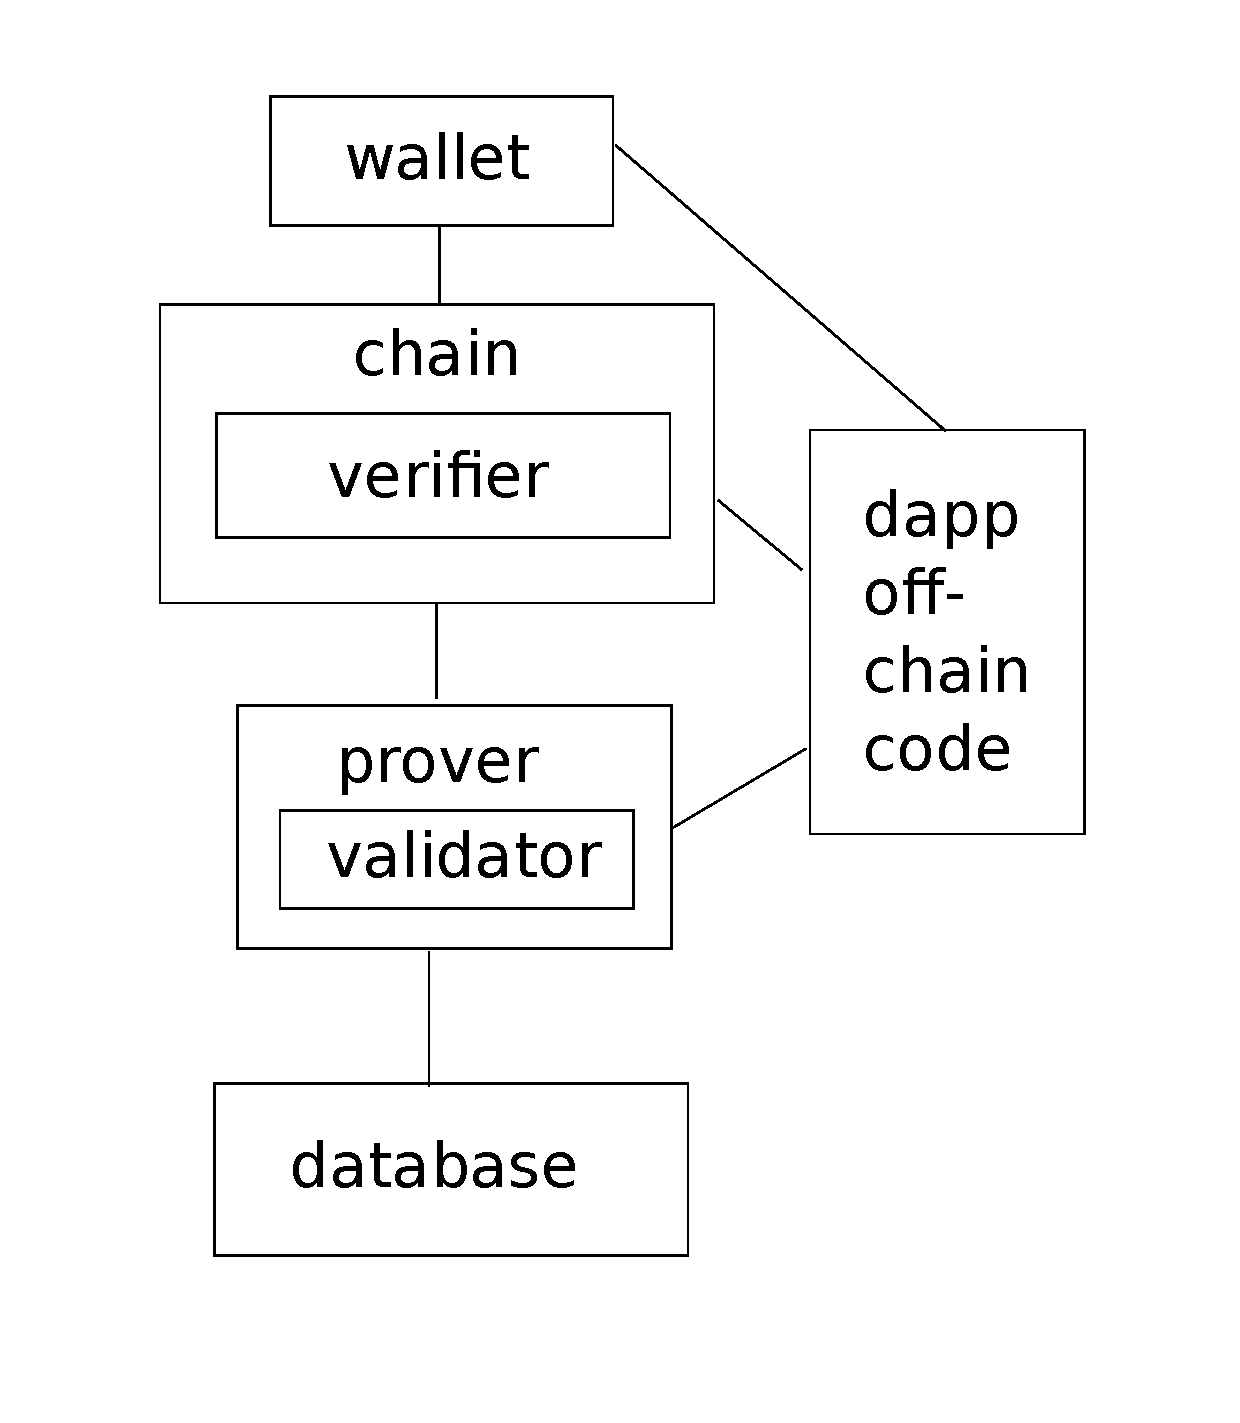
\includegraphics[width=1.0\columnwidth]{system-diagram.pdf}
	\caption{Key components of and related to Ardana Rollups.}
	\label{fig:system-diagram}
\end{figure}

Ardana Rollups provide an off-chain context in which smart contract validator code can run. Instead of being run to create transactions on the chain, in this context validator code is run to create transactions on the rollup and proofs that those transactions belong on the rollup.

It is important to keep two terms distinct here: \emph{verifier}\/ and \emph{validator}. ``Validator'' refers to a function which takes as input a transaction and produces as output a boolean value indicating whether or not the transaction satisfies the rules of a smart contract. ``Verifier'' refers to the smart contract validator which validates transactions over the rollup smart contract. The verifier is a validator, but other validators are not verifiers. In order to avoid confusion, let the term ``validator'' refer to the validator for some smart contract running on the rollup, as opposed to referring to the verifier (which runs on the blockchain).

Using Ardana Rollups complicates the process of developing a dapp (decentralized application) somewhat. The dapp must be aware of and control the movement of information from the chain to the rollup and back again. It must publish and subscribe to data not only on the chain but also on the rollup. The dapp interacts with the rollup by calling the prover API. The next section covers the processes involved in more detail.


\section{Processes}

There are three main processes involved in a dapp using Ardana Rollups: moving inputs from the chain to the rollup, posting transactions on the rollup, and moving outputs from the rollup to the chain. These processes are pictured in Figures~\ref{fig:process-a}, \ref{fig:process-b}, and \ref{fig:process-c}.

\begin{figure}
	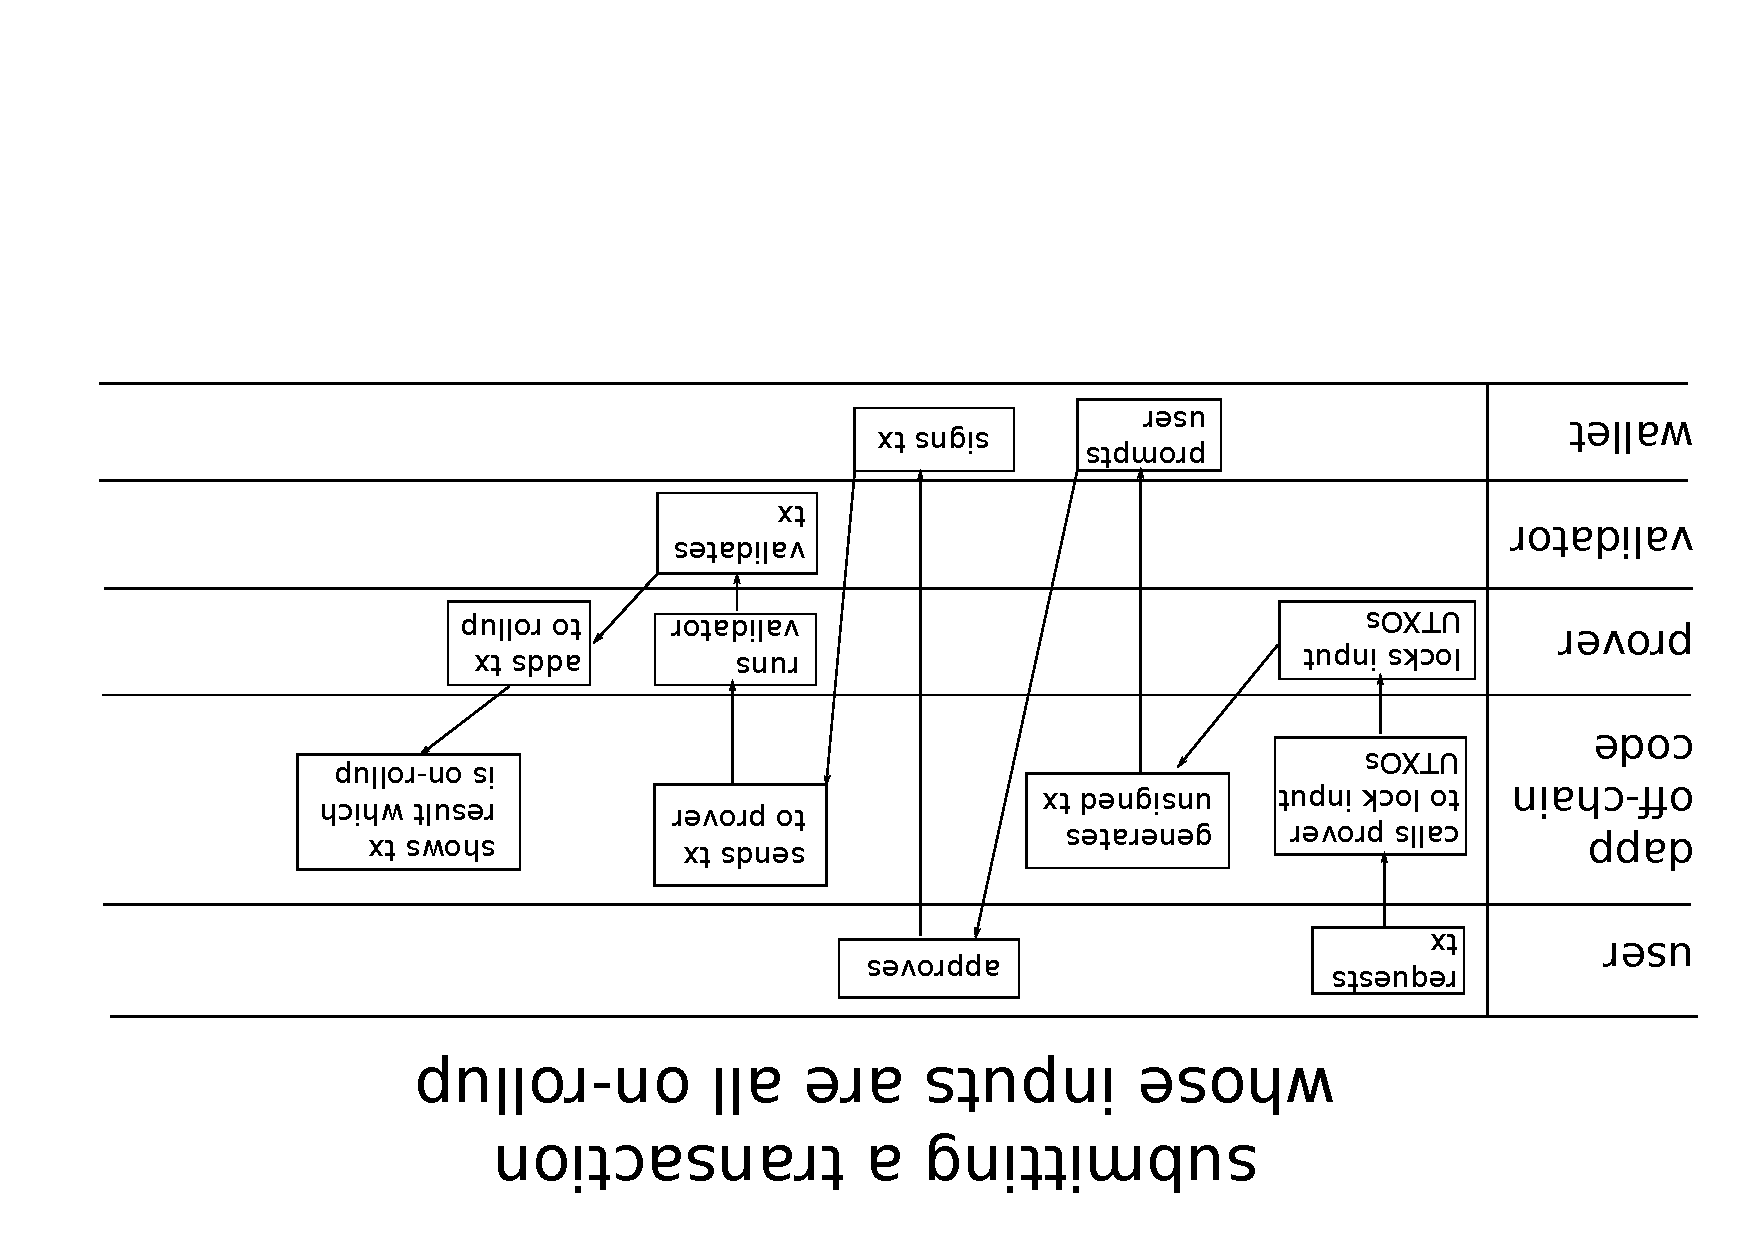
\includegraphics[angle=180,width=1.0\columnwidth]{process-diagram-a.pdf}
	\caption{Process of posting a transaction to a rollup.}
	\label{fig:process-a}
\end{figure}

\begin{figure}
	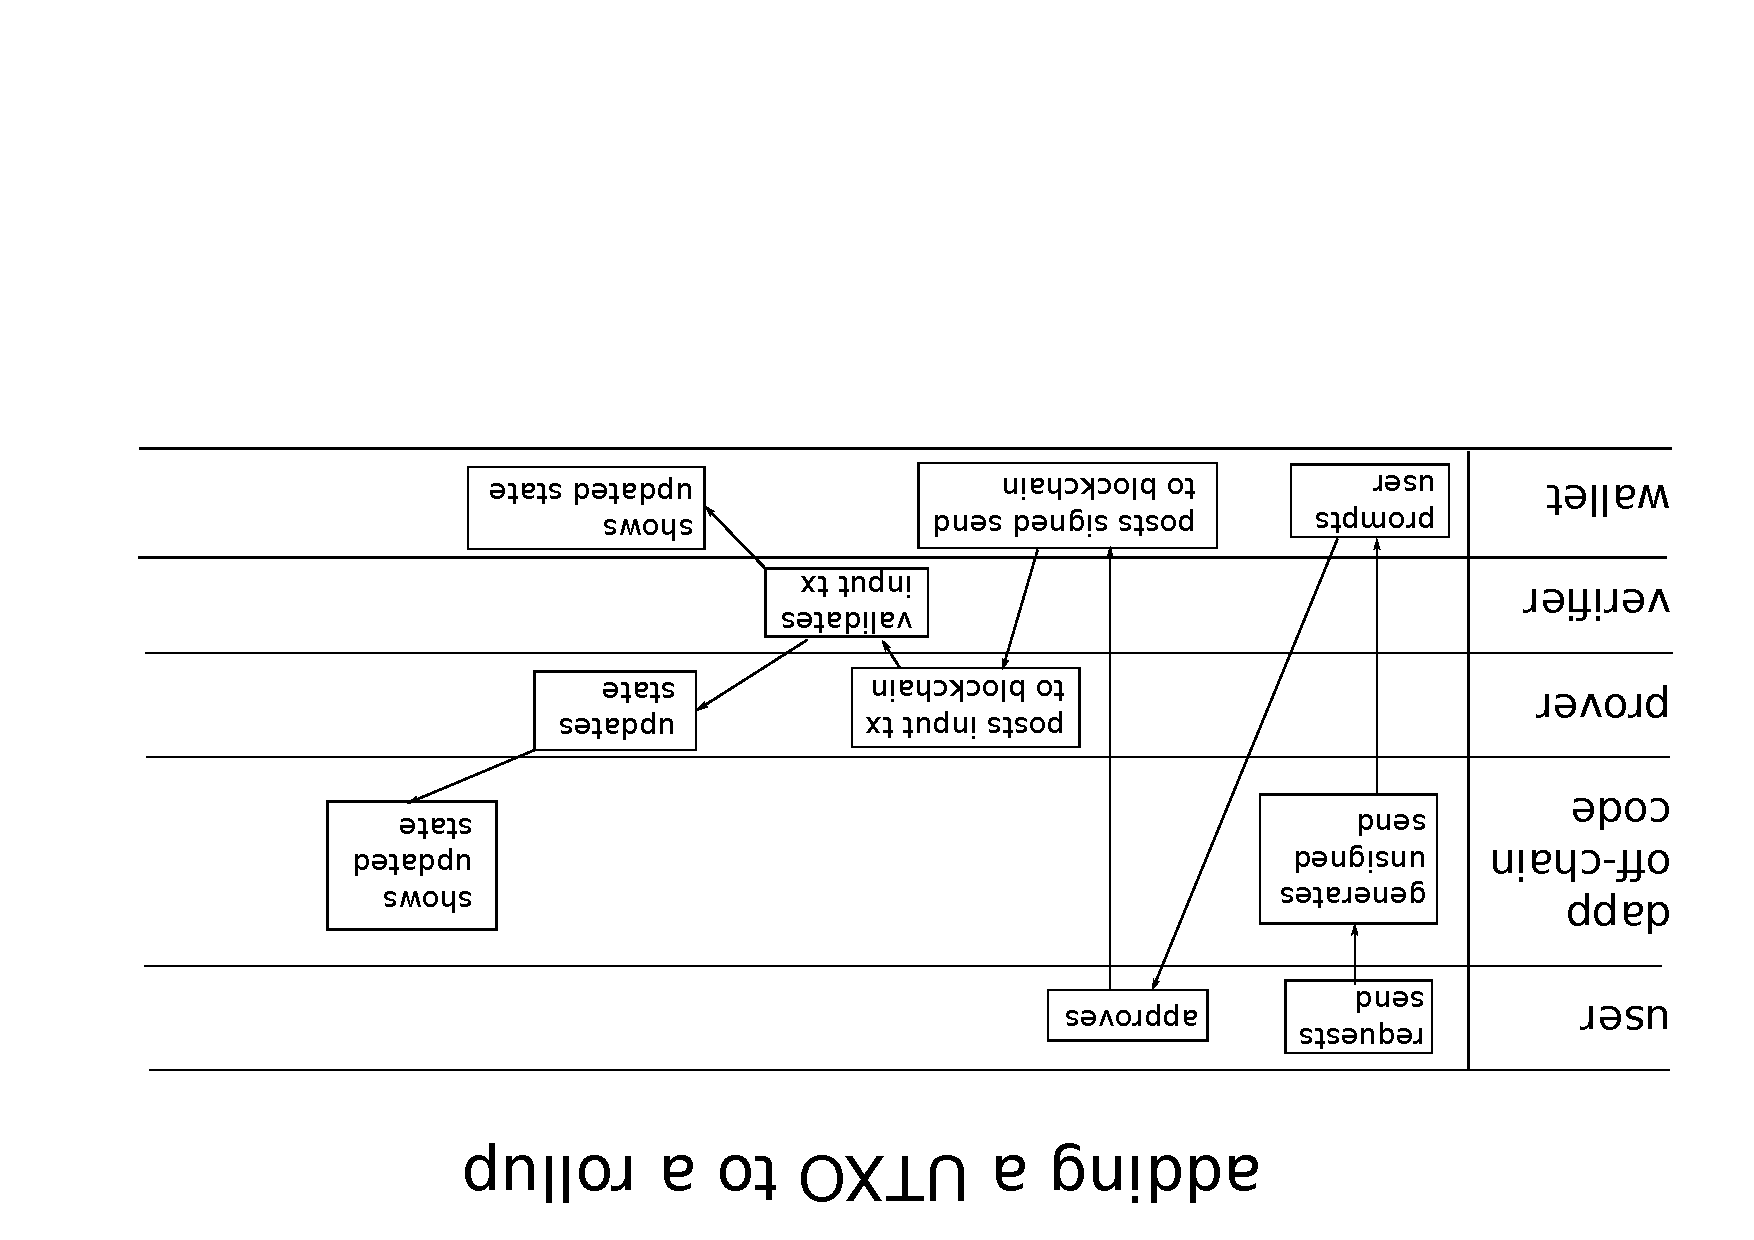
\includegraphics[angle=180,width=1.0\columnwidth]{process-diagram-b.pdf}
	\caption{Process of adding an input to a rollup.}
	\label{fig:process-b}
\end{figure}

\begin{figure}
	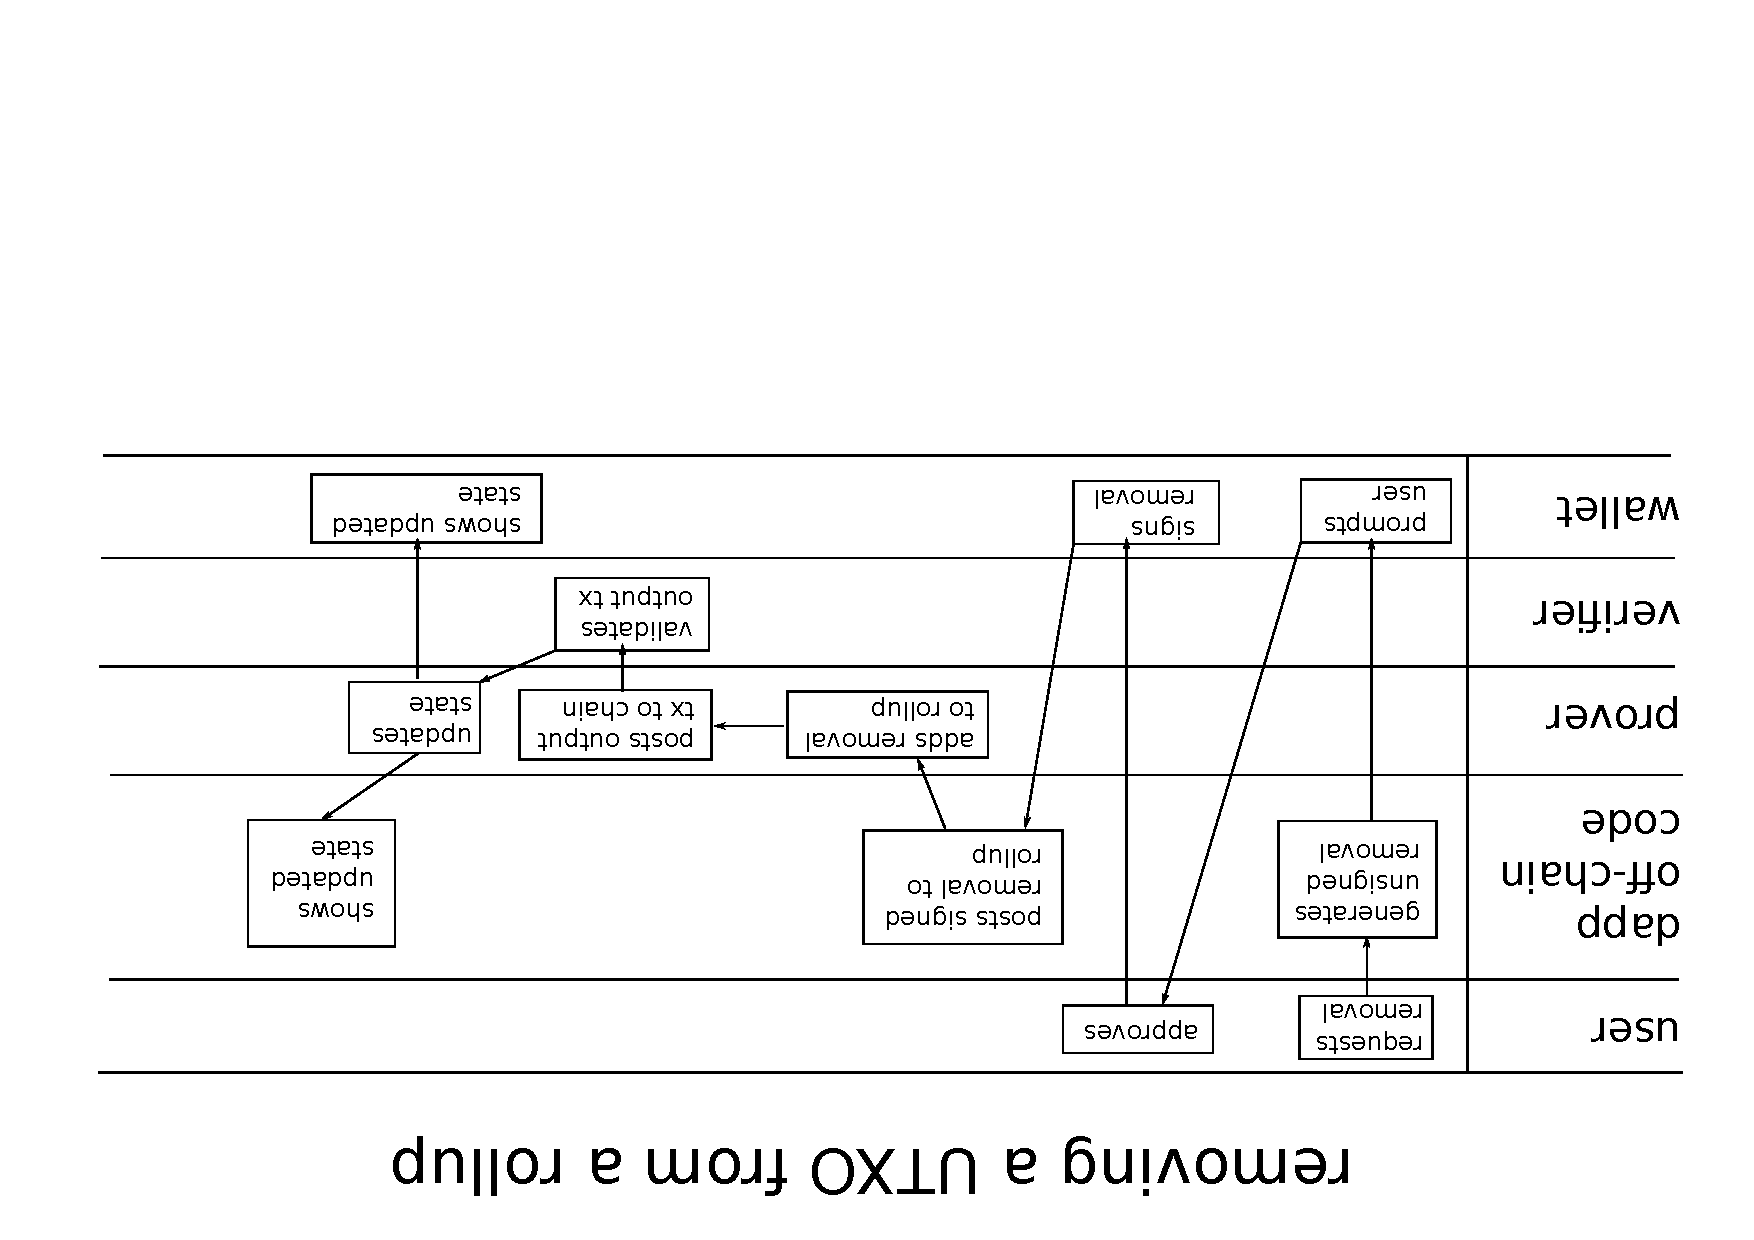
\includegraphics[angle=180,width=1.0\columnwidth]{process-diagram-c.pdf}
	\caption{Process of removing an output from a rollup.}
	\label{fig:process-c}
\end{figure}

\subsection{Process of posting a transaction to a rollup}

The first step of posting a transaction to a rollup is for the dapp code to call the prover API to lock the on-rollup input UTXOs. The purpose of this is to avoid resource contention problems which would prevent the transaction from going through. These locks should be temporary and expire automatically after a short time sufficient to complete the transaction. To avoid denial of service attacks based on this locking mechanism, the user requesting the transaction should be required to post collateral which will be lost if the locks expire without the inputs being used, or some other means should be used to prevent denial of service attacks based on this mechanism. The collateral can, for example, be one of the inputs being locked. Every transaction will have some monetary input, at least what is required to cover the transaction fee charged by the prover in order to cover the costs of proof generation. In response to the locking request, the prover provides some sort of key which the dapp may use to consume the on-rollup inputs. 

The next step is for the dapp to generate an unsigned transaction. The dapp sends the unsigned transaction to the user's wallet to be signed. The wallet signs the transaction with the user's approval. The dapp receives the signed transaction from the wallet and posts the transaction to the rollup by calling the prover API. The prover runs any validator scripts required for the transaction and generates a proof. The transaction, its outputs, and the proof are added to the rollup and the on-rollup inputs are marked as consumed. The dapp observes the rollup state changes via the prover API and makes them visible to the user.


\subsection{Process of adding an input to a rollup}

Adding an on-chain input to a rollup is essentially a two step process. First, the user sends the input to the rollup contract address. Second, the input gets picked up by an input transaction. The input transaction is an on-chain transaction which takes as input the rollup state UTXO and the inputs at the contract address which are to be added. It produces as output the new rollup state UTXO. The input transaction is signed by the prover. The rollup state UTXO contains the monetary values added to the rollup (in aggregate form, without tracking who owns what). It also contains whatever state data must be stored on-chain for the rollup contract.


\subsection{Process of removing an output from a rollup}

Removing an on-rollup output from the rollup and putting it on the chain is essentially a two step process. First, the user posts a removal transaction to the rollup. Second, the prover posts an output transaction to the chain and updates its internal state. An output transaction describes a set of output UTXOs and a proof (checked by the verifier contract) which shows that those outputs are lawful. One output transaction on-chain settles many removal transactions on-rollup.

\subsection{Authorization for updating the rollup}

The rollup contract will allow for two methods of authorizing a transaction with the rollup contract. These transactions should only be performed by authorized parties in order to prevent UTXO resource contention. The two methods of authorization are to sign the transaction with a signing key whose public key hash is stored in the rollup contract state, or to spend an authorization token (described in Section~\ref{sec:distribution-decentralization}.


\section{Distribution and decentralization of the prover}
\label{sec:distribution-decentralization}

Due to the high computational complexity of generating zkSNARK proofs which verify a large number of transactions, it will be necessary to make the prover a distributed system. By making use of recursive zkSNARK proofs, we can split the proof generation task into pieces which can be farmed out to different computers. This architecture assumes that it is possible to split the task of validating a sequence of transactions $\vec{t}$ (and generating the corresponding proof) into two subtasks which can done in parallel if the sequence can be split into two sequences $\vec{u}$ and $\vec{r}$, where some interpolation of the elements of $\vec{u}$ and $\vec{r}$ is equal to $\vec{t}$, and no transaction in $\vec{u}$ takes as input an output of a transaction in $\vec{r}$, and no transaction in $\vec{r}$ takes as input an output of a transaction in $\vec{u}$. This is assumed to be normally possible given dapp designs which are intended to make this possible. Thus we assume that we can split a sequence $\vec{t}$ of transactions into as many subsequences as are required to farm out the tasks of proof generation to as many computers as needed to make for sufficient throughput.

As per usual in designing a distributed system, the system should be designed to be fault tolerant, such that if one computer in the system fails, the system as a whole will continue to function as intended, without human intervention.

Distributing the prover is also a first step towards full decentralization of the prover. Full decentralization of the prover means that there is no computer, individual, or organization which is a single point of failure or a trusted entity in the prover protocol. Full decentralization of the prover is not in scope of the initial release, but is an eventual goal and commitment of the project. We are designing for an initial release which is not fully decentralized, and a smooth upgrade path (transparent from an end user perspective) to a fully decentralized prover.

In the distributed prover, one computer is at any given time designated as the leader of the system, responsible for coordinating all prover activities and for producing the final output transaction and posting it to the blockchain. In the centralized distributed prover, this leader is controlled and designated by Ardana (or more generally the organization which controls the signing key(s) for the rollup contract instance). In the decentralized prover, the leader is periodically determined by some leader election process to be designed later.

In the centralized prover, the prover is authorized to update the rollup contract instance by signing the transactions with the signing key(s) whose public key hashes are stored in the contract instance state. In the decentralized prover, another mechanism is needed, and the recommended mechanism is authorization tokens.

An authorization token is a token which allows its holder to perform an action. In this application, authorization tokens allow for the holder to update the rollup contract instance. The holder of an authorization token provides it as an input to a transaction to update the rollup contract instance, in lieu of signing the transaction. The transaction outputs the authorization token to some address. This authorization token output address is stored in the rollup contract instance state and can be set by a transaction signed using one of the authorized signing key(s).

The mechanism to update the authorization token output address is intended to be part of the smooth upgrade path from a centralized prover to a decentralized prover. For the upgrade path to be transparent to end users, it must not involve any change to the rollup contract, since a change to the rollup contract would necessitate moving funds from one contract to the other, and this cannot be done in a secure way without manual intervention by end users. We could build into the contract a provision allowing the funds in the rollup contract to be sent to a different contract using the authorized signing key(s), but this would open a security vulnerability where the person(s) in control of the signing key(s) could make off with the funds in the rollup contract. In the envisioned smooth upgrade path, we use a signed transaction with the rollup contract to set the authorization token output address to a contract address which handles the leader election process, ensuring that an authorization token makes it to the next elected leader.

In the decentralized version of the prover, there are additional security considerations to take into account. In the centralized version, we can assume that prover nodes (i.e., computers which take part in the distributed computing cluster constituting the prover) are not malicious. In the decentralized version, we cannot make this assumption, and thus we will need to do in depth security analysis to guard against acts of malicious prover nodes. To the greatest extent possible, we should guard against acts of malicious prover nodes by using zkSNARK proofs to ensure that such malicious acts did not occur. Where this does not work, we can also use an enforcement mechanism based on requiring prover node operators to post collateral which will be burned if the nodes act maliciously (and this depends on designing reliable mechanisms for detecting the occurrence of such malicious acts).


\section{Money trap avoidance}

One of the risks of ZK rollup solutions is denial of service. The prover is unable to post any outputs to the chain which are not lawful, but the prover is able to refuse service. Given that the prover is the only entity able to sign input and output transactions, if the prover stops operations, then the funds stored in the rollup contract would be lost. Another variant of this denial of service risk is that the prover might refuse service to certain market participants and not others, which could also cause those participants to lose money they put into the rollup contract. How can we mitigate these risks?

Ardana Rollups uses a model of exclusive access of one prover to a given rollup contract UTXO. The reason for this is to avoid resource contention where multiple provers contend for one rollup UTXO, which could result in performance issues and also complex situations where inputs are double spent, once by one prover and once by another prover. The latter situation would not result in actual double-spends on-chain, but it would preclude the possibility of both provers merging the outputs of their on-rollup transactions into the chain.

This exclusive access model (in contract to a permissionless model for using rollup UTXOs) leads to the mentioned money trap risk that occurs when a prover stops operating. In order to mitigate this risk, we can put an expiration time on a prover's exclusive access to the rollup UTXO. This means that the prover is expected to generate input and output transactions at some specified minimum frequency, and if this obligation is unmet, then the prover loses their exclusive access to the rollup UTXO and another prover is able to claim that exclusive access and retain it as long as they keep up with the obligation to post input and output transactions.

This idea of an expiring exclusive access to a rollup UTXO addresses the money trap risk which occurs when a prover stops operating. However, it does not address the money trap risk which occurs when a prover refuses service only to certain market participants. The latter risk will need to be addressed in a different way. The non-binding recommendation for solving this problem is to build into the rollup protocol a principle that input and output transactions must process inputs and outputs in a first-come first-served manner, meaning that the first inputs to be sent to the contract address are the first to be added to the rollup, and the first removal transactions posted to the rollup are the first to be processed in an output transaction.

The non-binding recommendation for implementing the first come, first served principle is to post transactions to a decentralized data structure such as a queue implemented as a decentralized conflict-free replicated data type (CRDT). Then we would enforce that the first come, first served principle is not violated by checking that leaders do not violate it and burning their collateral if they do, as part of the leader election protocol. It seems that it would be possible to check that this principle is followed as part of the zkSNARK proofs posted to the rollup verifier contract, but that would require us either to include enforcement of that principle as part of the initial verifier contract release, or to update the verifier contract post launch, which we want to avoid in order to allow for a smooth decentralization upgrade path transparent to end users.

Enforcing the first come, first served principle is out of scope of an initial release. For an initial release, we do not require a solution to the money trap risk associated with selective denial of service by a prover.


\section{Fees}

The fee structures for on-rollup and on-chain rollup transactions need to cover the costs of operating the system and also balance supply and demand to ensure availability of services. Defining the fee structures is out of scope of this document. For on-rollup transactions, it should be sufficient to charge fees which cover the operation costs of the rollup, since we should be able to scale to meet all demand for the on-rollup services. For on-chain rollup transactions, there is an upper limit to the throughput we can achieve pending further advances in the blockchain technology. Therefore, for on-chain rollup transactions, we will need to design a fee structure which includes ``availability surchages'' which serve to balance supply and demand in order to ensure availability of the services. The availability surcharges will be computed off-chain and charged by the rollup contract. Periodically, those fees will be collected by an authorized transaction with the rollup contract which sends the fees to a specified address (which can also be updated by another authorized transaction with the rollup contract).


\section{Database}

This architecture does not specify the nature of the database used to store the current rollup state and on-rollup transaction history. For the sake of transparency and fault tolerance, it may make sense to use a decentralized data store. For the sake of performance, it may make sense to use a traditional database such as PostgreSQL. It may make sense to use more than one database in order to address different considerations. It may make sense to store currently needed data in one database and archival data in another database.


\section{Verifer contract state data}

Here is a speculative, non-binding description of some state data which must be stored in the rollup UTXO.

\begin{enumerate}
	\item A nonce which gets incremented on every output transaction. The purpose of the nonce is to help ensure that on-rollup UTXOs are not used more than once. 
	\item A hash of all of the on-rollup UTXOs. The mentioned hash may be a recursive hash, i.e. a hash of UTXOs and a previous hash. The purpose of the state hash is to serve as an input to the proof checking algorithm.
	\item The public key hashes of the authorized signing key(s).
	\item The authorization token output address.
	\item The most recent time at which the prover posted an input transaction.
	\item The most recent time at which the prover posted an output transaction.
	\item The amount of collected availability surcharges currently stored in the rollup contract.
	\item The address to send collected availability surcharges to.
\end{enumerate}




\clearpage


\begin{thebibliography}{3}


	\bibitem{ethworks-20}
		Ethworks. \textit{Zero-Knowledge Blockchain Scalability}. Ethworks Reports, 2020. \url{https://ethworks.io/assets/download/zero-knowledge-blockchain-scaling-ethworks.pdf}

	\bibitem{visa}
		Visa. \textit{Power your retail business beyond the point of sale.} Accessed December 17, 2021. \url{https://usa.visa.com/run-your-business/small-business-tools/retail.html}

	\bibitem{chainweb}
		Will Martino, Monica Quaintance, and Stuart Popejoy. \textit{Chainweb: A Proof-of-Work Parallel-Chain Architecture for Massive Throughput.} DRAFT v15. \url{https://d31d887a-c1e0-47c2-aa51-c69f9f998b07.filesusr.com/ugd/86a16f_029c9991469e4565a7c334dd716345f4.pdf}

	\bibitem{dat}
		Maxwell Ogden, Karissa McKelvey, Mathias Buus Madsen, Code for Science. \textit{Dat - Distributed Dataset Synchronization And Versioning.} May 2017 (last updated: Jan 2018). \url{https://github.com/datprotocol/whitepaper/blob/master/dat-paper.pdf}

	\bibitem{ipfs}
		Juan Benet. \textit{IPFS - Content Addressed, Versioned, P2P File System.} Accessed Dec 22, 2021. \url{https://github.com/ipfs/ipfs/blob/master/papers/ipfs-cap2pfs/ipfs-p2p-file-system.pdf}


\end{thebibliography}



\end{document}
